\section{Постоянный электрический ток}

%1
\AddProb Найти сопротивление цепи между точками $А$ и $В$. Сопротивление каждого резистора известно и равно~$R$.

\begin{figure}[!h]
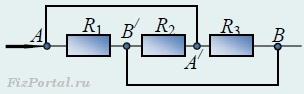
\includegraphics[scale=0.8]{1101DirectCurrentABCircuitLine.jpg}
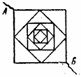
\includegraphics[scale=1]{1101DirectCurrentABCircuitStrange.jpg}
\end{figure}

\begin{figure}[!h]
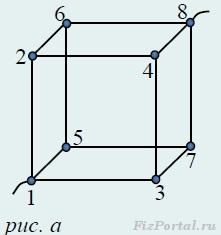
\includegraphics[scale=0.5]{1101DirectCurrentABCircuitCube.jpg}
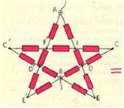
\includegraphics[scale=1]{1101DirectCurrentABCircuitStar.jpg}
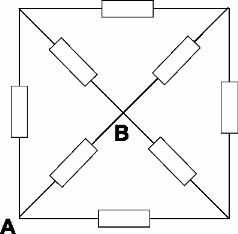
\includegraphics[scale=0.5]{1101DirectCurrentABCircuitSquare.jpg}
\end{figure}

\AddProb Сопротивления резисторов $R_1$~=~1~Ом, $R_2$~=~2~Ом, $R_3$~=~3~Ом, $R_4$~=~4~Ом. 
Напряжение источника тока $U$~=~1~В. Найдите ток, который течет через перемычку.

\begin{figure}[!h]
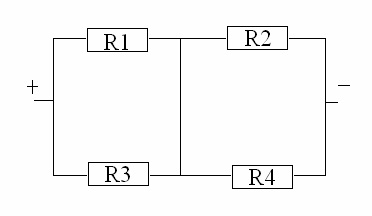
\includegraphics[scale=0.4]{1102DirectCurrentFourResistors.jpg}
\end{figure}

\begin{wrapfigure}{r}{3.5cm}
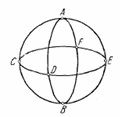
\includegraphics[scale=1]{1103DirectCurrentThreeRings.jpg}
\end{wrapfigure}

\AddProb Три одинаковых медных кольца радиуса $r$ соединены так, как показано на рисунке. 
Найдите сопротивление полученной таким образом фигуры, внешнее напряжение подано к точкам $A$ и $B$. 
Удельное сопротивление меди $\rho$, диаметр проволоки~$d$.

\AddProb Найдите эквивалентное сопротивление бесконечной цепочки (см рис), которая состоит из одинаковых резисторов сопротивлением $R$ каждый.

\begin{figure}[!h]
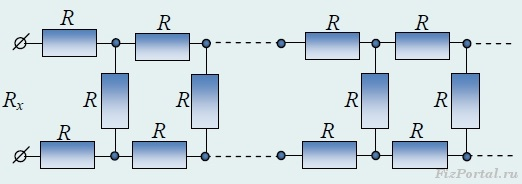
\includegraphics[scale=0.5]{1104DirectCurrentFourInfiniteCircuit.jpg}

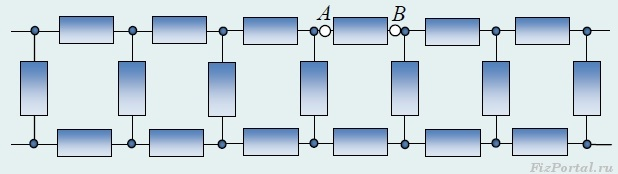
\includegraphics[scale=0.5]{1104DirectCurrentFourInfiniteCircuitAB.jpg}
\end{figure}

\begin{wrapfigure}{r}{2cm}
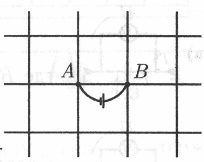
\includegraphics[scale=0.3]{1105DirectCurrentNet.jpg}
\end{wrapfigure}

\AddProb Из бесконечной проводящей квадратной сетки, каждое звено которой имеет сопротивление $R$, удалили одно звено $AB$. 
Найдите сопротивление сетки между точками $A$ и $B$.

%6
\AddProb Имеется $n$ клемм, каждая из которых соединена со всеми остальными клеммами одинаковыми проводниками сопротивлением $R$. 
Найдите сопротивление между любыми двумя клеммами.

\AddProb Электический чайник имеет две обмотки. При включении одной из них чайник вскипает через 10 мин, при включении другой -- через 15 мин. 
Через какое время чайник вскипит, если эти две обмотки включить вместе параллельно, последовательно?

\begin{wrapfigure}{r}{4cm}
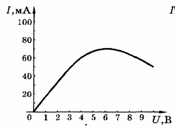
\includegraphics[scale=0.7]{1108DirectCurrentVDR.jpg}
\end{wrapfigure}

\AddProb На рисунке представлен график зависимости силы тока от напряжения на нелинейном резисторе. 
Определите силу тока в цепи при подключении этого резистора к источнику тока с напряжением 10 В и добавочным сопротивлением 100 Ом.

\begin{wrapfigure}{r}{2.5cm}
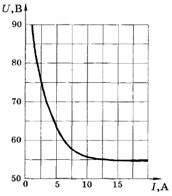
\includegraphics[scale=0.45]{1109DirectCurrentArcDischarge.jpg}
\end{wrapfigure}

\AddProb На рисунке приведен график зависимости напряжения на разрядном промежутке дугового разряда от тока. 
Дугу подключают  к источнику постоянного напряжения последовательно с резистором. 
При каком максимальном значении сопротивления резистора дуга может гореть при напряжении источника $U$~=~85~В?

\begin{wrapfigure}{r}{4cm}
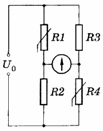
\includegraphics[scale=1]{1110DirectCurrentResistorsAndGalvanometor.jpg}
\end{wrapfigure}

\AddProb Схема, изображенная на рисунке, состоит из двух одинаковых резисторов $R_2$ и $R_3$ сопротивлением $R$ каждый 
и двух одинаковых нелинейных резисторов $R_1$ и $R_4$, вольтамперная характеристика которых имеет вид $U~=~\alpha~I$. 
При каком напряжении источника питания $U_0$ сила тока через гальванометр равна нулю?